\section{Future Work}


\subsection{Improve Robustness}
In this paper we have made many simplifications to the problem space just to make the placer easier to implement.
For example, our placer in its current state does not take advantage of \texttt{SLICEL}/\texttt{SLICEM} homogeneity and simply maps all SLICE \texttt{SiteInst}s onto \texttt{SLICEL}s. 
Recall that the SLICE Sites in Xilinx FPGAs typically come in a 75-25\% split between \texttt{SLICEL}s and \texttt{SLICEM}s. 
This means that we have rendered about 25\% of the CLB fabric unusable which will inevitably hurt wirelength minimization during placement since the \texttt{SiteInst}s must be spread over a larger area. 
Enabling \texttt{SLICEL}-\texttt{SLICEM} homogeneity can lead do greater logic density and consequently less total HPWL, but can make the packing process more complex and may contribute to higher routing congestion.

We can also add packing support for other Xilinx primitives such as the shift-register primitive \texttt{SRLx}, distributed RAM primitives \texttt{RAMSx}, or even \texttt{LATCH} primitives as discussed in \ref{sec:7_series}.
Adding support for additional primitives and macros will allow our placer to handle a wider range of HDL designs and will require deeper consideration of hardware constraints to ensure robustness.

In its current state, the prepacker and packer struggle to handle signals larger than 24-bits, especially when involved in DSP functions like addition and multiplication. 
In such designs, the Vivado synthesizer may synthesize long \texttt{CARRY4} chains with particular \texttt{EDIFHierPortInst} configurations which are currently not handled by our packer and lead to failures in the subsequent routing stage.
Further work is required to resolve these constraints in the packer.

\subsection{Force-Directed and Analytical Placement}
As mentioned previously, SA has largely been abandoned in favor of AP in SOTA placers, owing to SA's poor scalability and runtime.
Our placer follows a basic prepack-pack-place flow, where the final placement stage is driven by simulated annealing. 
In future work, we can retrofit this flow by replacing SA with AP in the final placement stage while fully reusing the prepacker and packer in its current state. 
We can still treat \texttt{SiteInst}s as the atomic objects to be placed and use analytical solvers to minimize the total HPWL of the nets between them. 

The following papers can serve as foundational references for building an AP placer or insight into the SOTA placers.
\begin{itemize}
    \item \emph{Analytical minimization of half-permieter wirelength} - \textbf{Kennings and Markov (2000)} \cite{AP_2000}.
    \item \emph{SimPL: an algorithm for placing VLSI circuits} - \textbf{Kim et al. (2013)} \cite{SimPL}.
    \item \emph{Analytical placement for heterogeneous FPGAs} - \textbf{Gort et al. (2012)} \cite{AP_2012}.
    \item \emph{Multi-Electrostatic FPGA Placement Considering SLICEL-SLICEM Heterogeneity, Clock Feasibility, and Timing Optimization} - \textbf{Jing et al. (2023)} \cite{MultiElectrostatic}.
    \item \emph{OpenPARF 3.0: Robust Multi-Electrostatics Based FPGA Macro Placement Considering Cascaded Macros Groups and Fence Regions} - \textbf{Jing et al. (2024)} \cite{OpenPARF}.
\end{itemize}





\subsection{Variations on Packing}
Our current placer follows a \textbf{Site-centric} approach that resembles that of the old Xilinx ISE - the predecessor to Vivado used in the 90s and 2000s.
These days, Vivado performs \textbf{BEL-centric} placement without necessarily locking \texttt{Cell}s into \texttt{Site}s, allowing for a higher granularity of movement of \texttt{Cell}s. 
Enabling BEL-centric moveme
nt as opposed to Site-centric movement can improve HPWL minimization, but will add much more complexity to the packing and placement process to ensure robustness with respect to hardware constraints.

There is no constraint that forces us to pack \texttt{Cells} into \texttt{SiteInst}s before placement or to follow a strict prepacking-packing-placement flow. 
After implementing a force-directed or analytical placer, we can begin to explore different packing and placement ordering like those studied in Wuxi et al. (2019) \cite{ExplicitPacking}.


\begin{equation}
    \boldsymbol{\Phi} (\vec{x}, \vec{y}) = \sum_{i, j} w_{i, j} ( |x_i - x_j| + |y_i - y_j| )
\end{equation}

{
    \centering
    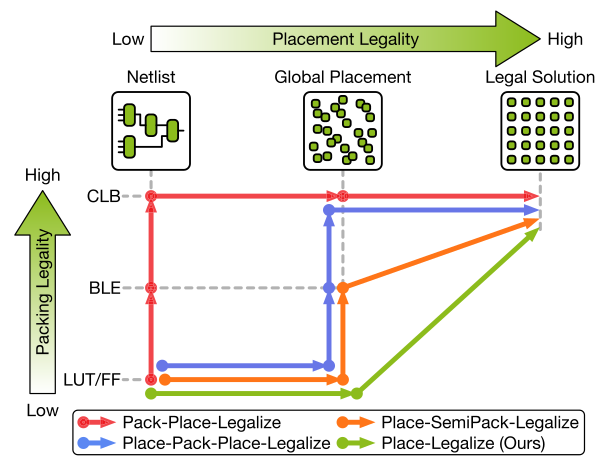
\includegraphics[width=\columnwidth]{figures/future_work/legalization.png}
    \captionof{figure}{Representative FPGA placement and packing flows. Figure taken from Wuxi et al. (2019), page 1 \cite{ExplicitPacking}}
}
\vspace{0.25cm}

\subsection{Add Hard Macro Support}






